\documentclass[conference]{IEEEtran}

\usepackage[utf8]{inputenc}
\usepackage{amsmath,amssymb}
\usepackage{graphicx}
\usepackage{cite}
\usepackage{amsthm}
\usepackage{hyperref}
\usepackage{subcaption} 

\newtheorem{claim}{Claim}
\newtheorem{definition}{Definition}



\begin{document}

\title{Quantum Error Correction (EE7001)}

\author{
    \IEEEauthorblockN{Tanay Bhat}
    \IEEEauthorblockA{
        Department of Electrical Engineering \\
        Indian Institute of Technology, Bombay \\
        Mumbai, India \\
        Email: 22b3303@iitb.ac.in
    }
    \and
    \IEEEauthorblockN{Jay Mehta}
    \IEEEauthorblockA{
        Department of Electrical Engineering \\
        Indian Institute of Technology, Bombay \\
        Mumbai, India \\
        Email: 22b1281@iitb.ac.in
    }
    \and
    \IEEEauthorblockN{Rajwardhan Toraskar}
    \IEEEauthorblockA{
        Department of Electrical Engineering \\
        Indian Institute of Technology, Bombay \\
        Mumbai, India \\
        Email: 22b0721@iitb.ac.in
    }
}

\maketitle

\begin{abstract}
    Quantum Error Correction (QEC) draws inspiration from classical error correction techniques to safeguard against errors. The 3-bit code serves as a starting point, being able to correct single bit-flip errors. This was then extended by Shor to the 9-bit code, which can correct both bit-flip and phase-flip errors. We shall also review bipartite purification protocols like the BBPSSW protocol and the DEJMPS protocol, which enhance the fidelity of entangled states which is crucial for quantum communication. 
\end{abstract}

\section{Introduction}
Quantum mechanics fundamentally changed our understanding of nature, revealing phenomena such as superposition and entanglement that defy classical intuition. Among these, entanglement has emerged as a cornerstone of modern quantum information science. Once regarded primarily as a conceptual puzzle, entanglement is now recognized as a key resource enabling quantum communication, computation, and cryptography. Experimental progress across diverse platforms—photons, trapped ions, atomic ensembles, superconducting circuits—has transformed theoretical proposals into tangible technologies. Yet, the practical realization of large-scale quantum systems remains limited by the inherent fragility of quantum coherence.

Every quantum system interacts inevitably with its surrounding environment, leading to noise and decoherence that degrade quantum states and destroy entanglement. Maintaining high-fidelity quantum information is therefore one of the most pressing challenges in the field. Two complementary strategies have been developed to combat these errors: entanglement purification and quantum error correction (QEC). Both aim to protect and restore the integrity of quantum information, albeit through different mechanisms.

Entanglement purification addresses the problem of distributing and maintaining entanglement over noisy quantum channels. By locally manipulating multiple imperfect copies of an entangled state and exchanging classical information, distant parties can probabilistically distill a smaller number of states with higher fidelity. Such purified entangled pairs can then serve as reliable channels for quantum teleportation, forming the foundation of quantum repeaters that enable long-distance quantum communication. These protocols, often relying on local operations and two-way classical communication, connect naturally with the principles of QEC—both can be seen as strategies to recover lost coherence and fidelity.

Quantum error correction, in contrast, provides an active and systematic framework for protecting unknown quantum states during computation or transmission. By encoding logical qubits into larger Hilbert spaces of multiple physical qubits, QEC enables the detection and correction of errors without direct measurement of the encoded information. The development of the first quantum codes in 1995 demonstrated that reliable, large-scale quantum computation was in principle possible. Subsequent advances introduced the stabilizer formalism, concatenated codes, and fault-tolerant architectures capable of withstanding realistic error rates below certain thresholds. Modern extensions—including subsystem and topological codes—offer powerful and scalable means of achieving fault-tolerant quantum processing.

Together, entanglement purification and quantum error correction constitute the theoretical backbone of fault-tolerant quantum information processing. They transform the unavoidable imperfections of physical systems into manageable errors, bridging the gap between fragile quantum hardware and the robust manipulation of information necessary for the future of quantum technologies.

This report will majorly summarise the findings of \cite{paper1} and \cite{paper2}.

\section{Quantum Errors}
We must note that coding based on data redundancy is not directly applicable to quantum information due to the no-cloning theorem, which prohibits the creation of identical copies of an arbitrary unknown quantum state. We also cannot perform direct measurements on qubits to detect errors, as this would collapse their superposition states. Additionally, quantum errors can be more complex as they are continuous in nature, unlike classical errors which are typically discrete (bit-flip or no bit-flip). QEC essentially relies on using data redundancy in a more sophisticated manner, encoding a single logical qubit into multiple physical qubits to protect against errors. Let us consider some common types of quantum errors.

\subsection{Types of Quantum Errors}

Consider the following two operations on a qubit:
\begin{itemize}
    \item \begin{equation}
        | \psi \rangle = \prod_{i = 1}^{N} I_i |0\rangle = |0 \rangle
    \end{equation}

    \item \begin{equation}
        | \psi \rangle = HIH |0\rangle = |0 \rangle
    \end{equation}
\end{itemize}

Note that these operations are functionally equivalent to $\sigma_I$ gate and are useful for understanding quantum errors.
\vspace{4pt}
\subsubsection{Coherent Errors}
These types of errors arise due to incorrect application of quantum gates. Such errors are systematic and can accumulate over time, leading to significant deviations from the intended quantum state. Consider the case where a small rotation is applied to a qubit. This results in the following state:

\begin{equation}
    | \psi \rangle = \prod_{i = 1}^{N} e^{i \epsilon \sigma_X} |0\rangle = \cos(N \epsilon ) |0\rangle + i \sin(N \epsilon) |1\rangle
\end{equation}

Hence $P(|0\rangle) = \cos^2(N \epsilon) \approx 1 - (N \epsilon)^2$ and $P(|1\rangle) = \sin^2(N \epsilon) \approx (N \epsilon)^2$. Hence error of order $O(\epsilon^2)$ has been introduced. We shall see that the 3-bit code can be used to supress such errors to $O(\epsilon^6)$.

\vspace{4pt}
\subsubsection{Environmental Decoherence}
Consider a system where the environment exists as orthogonal states $|e_0\rangle$ and $|e_1\rangle$. We also assume that the state of the environment flips if the coupled qubit is $|1\rangle$ else there is no change. Hence on application of the operation $HIH$ to the state $|0\rangle |e_0\rangle$, we get:

\begin{equation}
    | \psi \rangle = HIH |0\rangle |e_0\rangle = \frac{1}{2} (|0\rangle + |1\rangle) |e_0\rangle + \frac{1}{2} (|0\rangle - |1\rangle) |e_1\rangle
\end{equation}

This results in the following density matrix:

\begin{equation}
    \begin{aligned}
        \rho &= |\psi\rangle \langle \psi| \\
        &= \frac{1}{4} (|0\rangle + |1\rangle)(\langle 0| + \langle 1|) |e_0\rangle \langle e_0| \\
        &+ \frac{1}{4} (|0\rangle + |1\rangle)(\langle 0| - \langle 1|) |e_0\rangle \langle e_1| \\
        &+ \frac{1}{4} (|0\rangle - |1\rangle)(\langle 0| + \langle 1|) |e_1\rangle \langle e_0| \\
        &+ \frac{1}{4} (|0\rangle - |1\rangle)(\langle 0| - \langle 1|) |e_1\rangle \langle e_1|
    \end{aligned}
\end{equation}

We can trace out the environment to get the reduced density matrix of the qubit as:

\begin{equation}
    \rho_q = \frac{1}{2} (|0\rangle \langle 0| + |1\rangle \langle 1|)
\end{equation}

Hence on measurement of the qubit, we get $|0\rangle$ or $|1\rangle$ with equal probability and hence the qubit has completely decohered.

\vspace{4pt}
\subsubsection{Loss, Leakage, Measurement and Initialization Errors}

In addition to coherent control errors and environmental decoherence, practical quantum devices experience several other imperfections such as qubit loss, leakage, measurement inaccuracies, and imperfect initialization. These can be modeled either coherently or incoherently depending on their physical origin.

\textbf{Measurement Errors:} Measurement noise is commonly modeled as an incoherent process. Two equivalent formulations are typically used.

\textit{(i) POVM Model:} The measurement operators are
\begin{equation}
        \begin{aligned}
            F_0 &= (1-p_M)|0\rangle\langle 0| + p_M |1\rangle\langle 1| \\
            F_1 &= (1-p_M)|1\rangle\langle 1| + p_M |0\rangle\langle 0|
        \end{aligned}
\end{equation}
where $p_M$ denotes the measurement error probability. Since $F_i^2 \neq F_i$, the operators are non-projective. The corresponding outcome probabilities are
\begin{equation}
\mathrm{Tr}(F_0\rho) = (1-p_M)\mathrm{Tr}(A_0\rho) + p_M \mathrm{Tr}(A_1\rho),
\end{equation}
\begin{equation}
\mathrm{Tr}(F_1\rho) = (1-p_M)\mathrm{Tr}(A_1\rho) + p_M \mathrm{Tr}(A_0\rho),
\end{equation}
where $A_0 = |0\rangle\langle 0|$ and $A_1 = |1\rangle\langle 1|$.  
The post-measurement state is given by
\begin{equation}
\rho \rightarrow \frac{M_i \rho M_i^\dagger}{\mathrm{Tr}(F_i\rho)}, \quad
M_0 = \sqrt{1-p_M}|0\rangle\langle 0| + \sqrt{p_M}|1\rangle\langle 1|.
\end{equation}
Thus, the measured qubit remains in a superposed state rather than collapsing completely into a basis vector.

\textit{(ii) Bit-Flip Channel Model:} Alternatively, measurement error can be modeled as a bit-flip with probability $p_M$, followed by an ideal measurement:
\begin{equation}
\rho \rightarrow \rho' = (1-p_M)\rho + p_M X\rho X,
\end{equation}
where $X$ is the Pauli-$X$ operator. Both models yield the same measurement statistics but differ in the post-measurement states. The POVM model leaves residual coherence, while the bit-flip model projects the state directly onto $|0\rangle$ or $|1\rangle$.  
For instance, for $|\psi\rangle = \tfrac{1}{\sqrt{2}}(|0\rangle + |1\rangle)$, the POVM model produces $\sqrt{1-p_M}|0\rangle + \sqrt{p_M}|1\rangle$, whereas the bit-flip model yields $|0\rangle$.  
In practical systems, since qubits are reinitialized immediately after measurement, either approach provides equivalent results for simulation purposes.

\textbf{Qubit Loss:} Qubit loss refers to the disappearance of the physical information carrier from the system. It can be modeled by tracing out the lost subsystem:
\begin{equation}
\rho \rightarrow \mathrm{Tr}_i(\rho),
\end{equation}
which effectively reduces the Hilbert space dimension by a factor of two.  
Since standard QEC protocols assume that qubits remain physically accessible, loss correction typically requires a non-demolition detection mechanism to verify qubit presence without perturbing its logical state. The detection of a loss event can serve as a herald, allowing the replacement of the missing qubit and improving overall error resilience.

\textbf{Initialization Errors:} Initialization imperfections can manifest as either incoherent or coherent errors. Incoherent initialization can be represented as a probabilistic mixture:
\begin{equation}
\rho_i = (1-p_I)|0\rangle\langle 0| + p_I |1\rangle\langle 1|,
\end{equation}
whereas a coherent initialization error corresponds to preparing a slightly rotated pure state:
\begin{equation}
|\psi_i\rangle = \alpha|0\rangle + \beta|1\rangle, \quad |\alpha|^2 + |\beta|^2 = 1, \quad |\beta|^2 \ll 1.
\end{equation}
Both forms increase the probability of incorrect measurement outcomes, effectively lowering the fidelity of qubit preparation.

\textbf{Qubit Leakage:} Leakage occurs when the system state escapes the computational subspace $\{|0\rangle, |1\rangle\}$ into higher excited levels such as $|2\rangle$. In an ion-trap qubit, for example, an imperfect pulse may produce
\begin{equation}
U|0\rangle = \alpha|0\rangle + \beta|1\rangle + \gamma|2\rangle.
\end{equation}
Such leakage violates the two-level approximation and introduces additional decoherence if the higher level $|2\rangle$ decays rapidly.  
Mitigation strategies include:  
(i) Non-demolition verification to ensure the qubit remains within the computational manifold, and  
(ii) Pulse refocusing sequences that coherently return leaked population back to the logical subspace.  

Leakage can arise from both dynamic control errors and fabrication imperfections. The latter can be mitigated by post-fabrication characterization and exclusion of faulty qubits, reducing the necessity for active leakage correction.

\textbf{Summary:} Loss, leakage, measurement, and initialization errors all contribute to the non-ideal behavior of quantum devices. Accurate modeling of these processes as coherent or incoherent quantum channels is crucial for the development of reliable quantum error correction and fault-tolerant architectures.


\section{Entanglement Purification and QEC}
We can transmit quantum information over a channel using teleportation. Recall that teleportation involves the users Alice and Bob to share a maximally entangled state (like $| \phi^+ \rangle$) and then Alice performing a Bell measurement on her half of the entangled state and the qubit to be transmitted. She then sends the result of the measurement to Bob over a classical channel, who then applies a unitary operation on his half of the entangled state to get the original qubit. However in the presence of a noisy channel, the act of sending one half of the entangled state to Bob will result in a noisy non-maximally entagled state. This in turn affects the fidelity of the teleported qubit. To combat this, multiple copies of the noisy entangled state are produced and then purified using entanglement purification which essentially means increasing entanglement of a few copies. \par

These purification protocols can be categorized as distillation, recurrence and pumping schemes. Distillation involves applying local operations to multiple copies of noisy states to generate a few states with higher fidelity. The latter two involved repeating the purification step multiple times to improve the fidelity of states.
\section{3-bit and 9-bit Shor Code}
\subsection{The 3-Qubit Bit-Flip Code}
\subsubsection{Why the 3-Qubit Code Works}

The 3-qubit bit-flip code protects a single logical qubit against a single $\sigma_x$ (bit-flip) error by encoding it redundantly across three physical qubits. The logical basis states are:

\begin{equation}
|0\rangle_L = |000\rangle, \quad |1\rangle_L = |111\rangle
\end{equation}

An arbitrary qubit state
\begin{equation}
|\psi\rangle = \alpha |0\rangle + \beta |1\rangle
\end{equation}
is mapped to the encoded state
\begin{equation}
|\psi\rangle_L = \alpha |0\rangle_L + \beta |1\rangle_L = \alpha |000\rangle + \beta |111\rangle.
\end{equation}

The code works because the minimum Hamming distance between the codewords is $d = 3$, meaning that at least three bit flips are required to transform $|0\rangle_L \leftrightarrow |1\rangle_L$. This allows correction of a single bit-flip error, as the corrupted state remains closer to the original logical state. The number of correctable errors $t$ is related to $d$ by:
\begin{equation}
t = \left\lfloor \frac{d-1}{2} \right\rfloor = 1.
\end{equation}

\subsubsection{How the 3-Qubit Code Works}

Error correction uses two ancilla qubits to extract a \textit{syndrome} without measuring the logical qubit directly. After applying CNOT gates to check parity, the ancilla measurement reveals which, if any, qubit has flipped. For instance, the ancilla measurement outcomes and corresponding corrections are:

\begin{equation}
\begin{aligned}
00 &\quad \text{No error} \\
01 &\quad \sigma_x \text{ on qubit 3} \\
10 &\quad \sigma_x \text{ on qubit 2} \\
11 &\quad \sigma_x \text{ on qubit 1}
\end{aligned}
\end{equation}

For coherent rotation errors $U = \exp(i \epsilon \sigma_x)$ on each qubit, the total error operator is
\begin{equation}
E = U^{\otimes 3} = (\cos \epsilon\, \sigma_I + i \sin \epsilon\, \sigma_x)^{\otimes 3} = c_0 \sigma_I \sigma_I \sigma_I + c_1 (\sigma_x \sigma_I \sigma_I + \dots) + c_2 (\dots) + c_3 \sigma_x \sigma_x \sigma_x,
\end{equation}
with
\begin{equation}
c_0 = \cos^3 \epsilon, \quad c_1 = i \cos^2 \epsilon \sin \epsilon, \quad c_2 = -\cos \epsilon \sin^2 \epsilon, \quad c_3 = -i \sin^3 \epsilon.
\end{equation}

After error correction and ancilla measurement, the encoded qubit fidelity is improved from
\begin{equation}
F_{\text{unencoded}} = \cos^2 \epsilon \approx 1 - \epsilon^2
\end{equation}
to
\begin{equation}
F_{\text{encoded}} \approx 1 - \epsilon^6
\end{equation}
if no error is detected.

\subsection{The 9-Qubit Shor Code}

\subsubsection{Why the 9-Qubit Code Works}

The 9-qubit Shor code extends the 3-qubit repetition code to correct both single bit-flip ($\sigma_x$) and phase-flip ($\sigma_z$) errors. The logical states are

\begin{equation}
\begin{aligned}
|0\rangle_L &= \frac{1}{2\sqrt{2}} (|000\rangle + |111\rangle)(|000\rangle + |111\rangle)(|000\rangle + |111\rangle), \\
|1\rangle_L &= \frac{1}{2\sqrt{2}} (|000\rangle - |111\rangle)(|000\rangle - |111\rangle)(|000\rangle - |111\rangle).
\end{aligned}
\end{equation}

Each block of three qubits can correct a single $\sigma_x$ error, while phase errors are corrected by comparing relative phases between the three blocks. The code is \textit{degenerate}, meaning different errors may have the same effect on the logical state, allowing more flexibility in correction.

\subsubsection{How the 9-Qubit Code Works}

Bit-flip correction is applied independently to each 3-qubit block using the same parity check as in the 3-qubit code. Phase-flip correction uses CNOT gates to compare the signs between blocks. For example, a phase-flip $\sigma_z$ on a qubit changes the relative phase in its block, which is detected by the inter-block parity check.

The error operator for coherent rotations can be generalized as
\begin{equation}
E = \bigotimes_{i=1}^{9} (\cos \epsilon\, \sigma_I + i \sin \epsilon\, \sigma_x),
\end{equation}
and the combination of X and Z correction circuits restores the logical qubit to a higher fidelity state than the unencoded qubit. The Shor code is thus a full quantum error correcting code capable of correcting arbitrary single-qubit errors.



\section{Bipartite Purification Protocols}
We shall noe discuss the main bipartite purification protocols - the BBPSSW protocol and the DEJMPS protocol which have been outlined in \cite{paper2}. Before we do that we shall define the following:

\begin{equation}
    | \phi_{00} \rangle = \frac{1}{\sqrt{2}} (|0\rangle_z |0\rangle_x + |1\rangle_z |1\rangle_x)
\end{equation}

Here $|0\rangle_z$ and $|1\rangle_z$ are the eigenstates of $\sigma_Z$ and $|0\rangle_x$ and $|1\rangle_x$ are the eigenstates of $\sigma_X$ with eigenvalues $\pm 1$ respectively. The other Bell states can be generated as follows:

\begin{equation}
    | \phi_{ij} \rangle = \sigma_z^i \sigma_z^j | \phi_{00} \rangle
\end{equation}

Here i, j control the operation on the first and second qubit respectively. We should also note that these bell states are eigenvectors for the operators

\begin{equation}
    K_1 = \sigma_x^i \sigma_z^j, \quad K_2 = \sigma_z^i \sigma_x^j
\end{equation}

with eigenvalues $(-1)^i$ and $(-1)^j$ respectively. We may use these bell bases vectors to express a mixed state $\rho_{AB}'$ shared between Alice and Bob as follows:

\begin{equation}
    \rho_{AB}' = \sum_{k_1, k_2, j_1, j_2 = 0}^{1} \lambda_{k_1 k_2 j_1 j_2} | \phi_{k_1 k_2} \rangle \langle \phi_{j_1 j_2} |
\end{equation}

Consider the operators $\{I, K_1, K_2, K_1 K_2\}$. If we apply say $K_1$ on the basis states $| \phi_{k_1 k_2} \rangle$, we get back the same state if $k_1 = 0$ and we get $- | \phi_{k_1 k_2} \rangle$ if $k_1 = 1$. Hence all off-diagonal terms (diagonal entries are those where $k_1 = j_1$ and $k_2 = j_2$) in $\rho_{AB}'$ will assume the form $(-1)^{k_1 \oplus j_1} | \phi_{k_1 k_2} \rangle \langle \phi_{j_1 j_2} |$. Now if we consider probabilistic application of $K_1$ then the density operator will be transformed as follows:

\begin{equation}
    \rho_{AB}' \rightarrow (1-p)\rho_{AB}' + p K_1 \rho_{AB}' K_1^\dagger
\end{equation}

And for $p = 0.5$, we see that all off diagonal terms where $k_1 \neq j_1$ will vanish. Similarly we can cancel out the other off-diagonal terms by application of an appropriate operator. We shall now claim the following.

\begin{claim}
    The procedure outlined above does not affect the fidelty of the state.
\end{claim}

\begin{proof}
    Let $\rho' = \sum_{k \in K} \alpha_k k \rho k^\dagger$ where $K$ is the above set of operators and $\alpha_k$ are probabilities. Then we have:
    \begin{equation}
        \begin{aligned}
            F(\rho') &= \langle \phi_{00} | \rho' | \phi_{00} \rangle \\
            &= \sum_{k \in K} \alpha_k \langle \phi_{00} | k \rho k^\dagger | \phi_{00} \rangle \\
            &= \sum_{k \in K} \alpha_k \langle \phi_{00} | \rho | \phi_{00} \rangle \\
            &= F(\rho)
        \end{aligned}
    \end{equation}
    This is because $k | \phi_{00} \rangle = | \phi_{00} \rangle$ for all $k \in K$.
\end{proof}

\cite{paper2} also highlights that we can indeed reduce this further so that only the diagonal terms remain. This is done by applying the operators of the form $U \otimes HU^*H$ as it leaves $| \phi_{00} \rangle$ invariant upto a phase and transforms the other bell states.

\begin{claim}
    Operators of the form $U \otimes HU^*H$ leave $| \phi_{00} \rangle$ invariant upto a phase.
\end{claim}

\begin{proof}
    Consider the state $| \phi^+ \rangle = \frac{1}{\sqrt{2}} (|0\rangle_z |0\rangle_z + |1\rangle_z |1\rangle_z)$. We can represent the defined bell states $| \phi_{00} \rangle$ in terms of $| \phi^+ \rangle$ as follows:

    \begin{equation}
        | \phi_{00} \rangle = (I \otimes H) | \phi^+ \rangle
    \end{equation}

    Also note 
\end{proof}

\section{Implementation and Experimental Results}
In terms of implementation, we have used Qiskit to simulate the 3-bit and 9-bit Shor code. The codes can be found in the Codes directory of the \href{https://github.com/jaymehta132/QuantumErrorCorrection-EE7001}{repository}. The methodology used and results obtained are mentioned as follows: 
\subsection{3-bit Code for X error}

\href{https://github.com/jaymehta132/QuantumErrorCorrection-EE7001/blob/main/Codes/scripts/3bitCode.py}{This code} implements the three-qubit bit-flip quantum error correction protocol, which protects a logical qubit against a single bit-flip error by encoding, detecting, and correcting errors using quantum gates and measurements. The process begins by encoding a logical qubit into three physical qubits through a Hadamard gate and two CNOT gates, creating an entangled state that distributes the quantum information. A deliberate bit-flip error is then introduced on one of the physical qubits to simulate noise. To detect and locate the error, two ancilla qubits are entangled with the data qubits using CNOT gates, and their measurement reveals the error syndrome without collapsing the encoded quantum information. Based on the measured syndrome, a conditional correction is applied: the corresponding qubit is flipped if an error is detected, ensuring the logical state is restored. Finally, the logical qubit is decoded back to a single qubit and measured to verify successful error correction. The simulation results are visualized and saved, demonstrating the effectiveness of the protocol in correcting single bit-flip errors while preserving quantum coherence.

\begin{figure}[h]
    \centering
    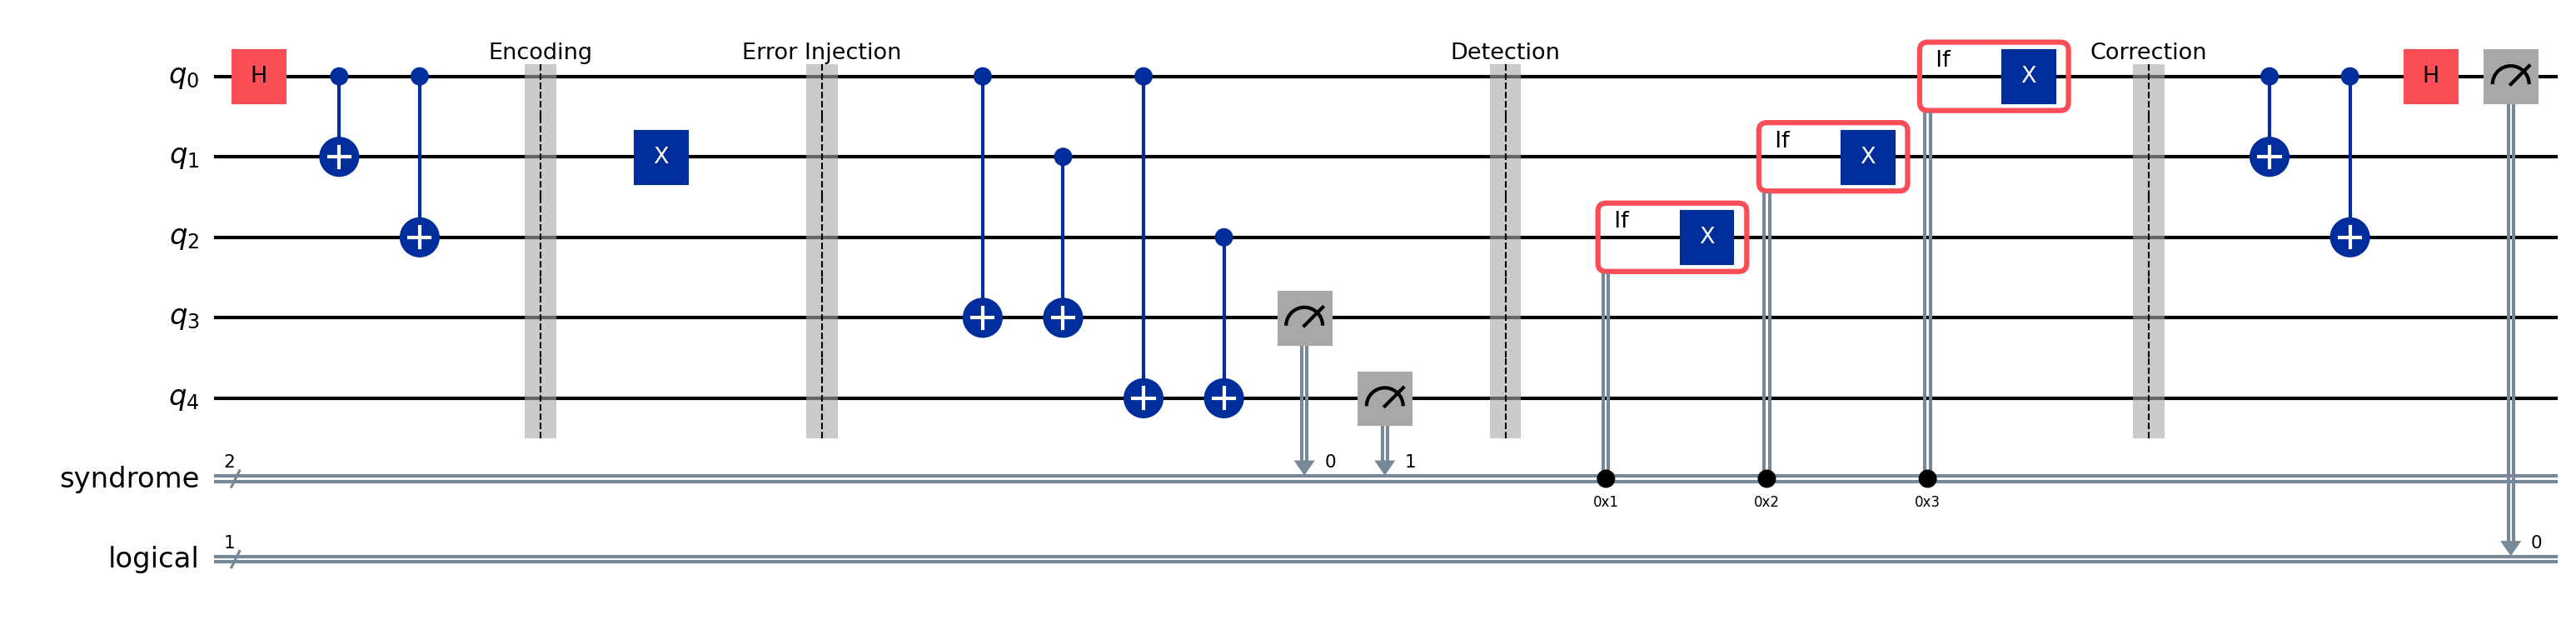
\includegraphics[width=0.45\textwidth]{../Codes/results/3bitCode/3bitCodeCircuit.png}
    \caption{3-bit Code Circuit for X error}
    \label{fig:3bitCodeCircuit}
\end{figure}

The first Hadamard gate is to convert the basis from Z-basis to X-basis. The next two CNOT gates are used to encode the qubit. The X gate is used to introduce an error in the second qubit. The next four CNOT gates are used to detect the error using two ancilla qubits. The measurement of the ancilla qubits gives us the error syndrome which is then used to correct the error using conditional X gates. Finally, we decode the qubit using two CNOT gates and a Hadamard gate and measure it. 

The results obtained are as follows:
\begin{figure}[h]
    \centering
    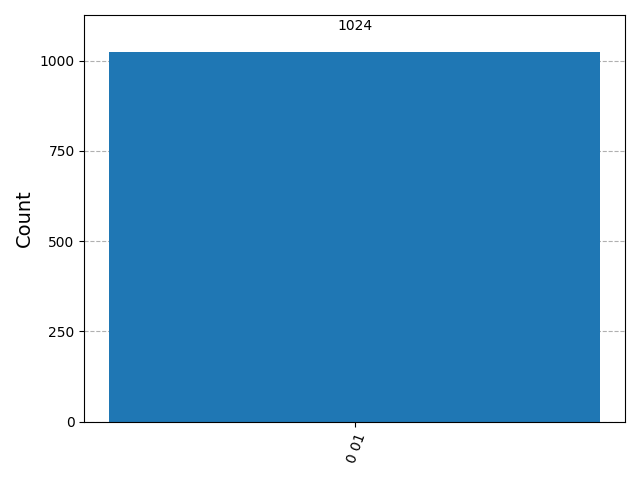
\includegraphics[width=0.45\textwidth]{../Codes/results/3bitCode/3bitCodeHistogram.png}
    \caption{3-bit Code Results for X error}
    \label{fig:3bitCodeResults} 
\end{figure}

The last two bits in the histogram represent the ancilla qubits used for error detection. The first bit represents the output of the measurement of the corrected qubit in the X-basis. The results show that the output is "001" with a probability of 1, indicating that the error correction was successful and the logical qubit was restored to its original state. 

\subsection{3-bit Code for Phase error}
\href{https://github.com/jaymehta132/QuantumErrorCorrection-EE7001/blob/main/Codes/scripts/3bitPhaseEC.py}{This code} simulates the effectiveness of the three-qubit bit-flip quantum error correction code in suppressing small coherent errors, specifically single-qubit X rotations of magnitude $\epsilon$. It first calculates the fidelity of an unencoded qubit state $|0\rangle$ after the error, showing that the fidelity drops by approximately $\epsilon^2$. Next, it encodes the state into three qubits using CNOT gates, applies the same error to all three data qubits, and simulates syndrome extraction using two ancilla qubits via further CNOT gates. The code then post-selects the component where no error is detected (syndrome '00'), normalizes this state, and decodes it back to a single qubit. The fidelity of the corrected, decoded state is calculated and shown to be suppressed to order $\epsilon^6$, demonstrating the power of quantum error correction: the probability of error is reduced from quadratic to sixth order in $\epsilon$. The code outputs and compares both fidelities, confirming that the encoded and corrected state retains much higher fidelity than the unencoded state, as expected from theory.
\begin{figure}[h!]
    \centering

    \begin{subfigure}[b]{0.3\columnwidth}
        \centering
        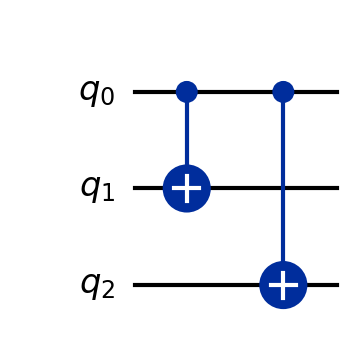
\includegraphics[width=\textwidth]{../Codes/results/3bitPhaseEC/EncodingCircuit.png}
        \caption{Encoding Circuit}
        \label{fig:3bitPhaseECCircuit}
    \end{subfigure}
    \hfill
    \begin{subfigure}[b]{0.3\columnwidth}
        \centering
        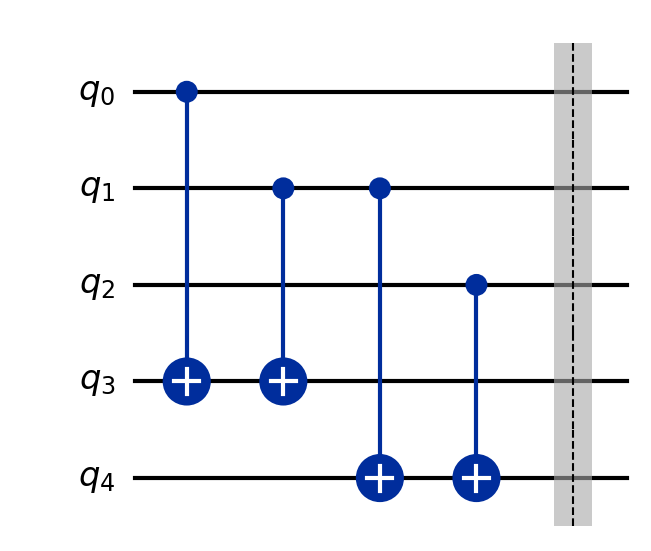
\includegraphics[width=\textwidth]{../Codes/results/3bitPhaseEC/SyndromeMeasurementCircuit.png}
        \caption{Syndrome Measurement Circuit}
        \label{fig:3bitPhaseDecodingCircuit}
    \end{subfigure}
    \hfill
    \begin{subfigure}[b]{0.3\columnwidth}
        \centering
        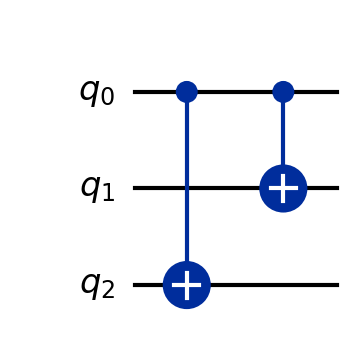
\includegraphics[width=\textwidth]{../Codes/results/3bitPhaseEC/DecodingCircuit.png}
        \caption{Decoding Circuit}
        \label{fig:3bitPhaseAncillaCircuit}
    \end{subfigure}

    \caption{3-bit Code Circuits for Phase error}
    \label{fig:three_images}
\end{figure}

The first circuit (Fig. \ref{fig:3bitPhaseECCircuit}) encodes the qubit using two CNOT gates. The second circuit (Fig. \ref{fig:3bitPhaseDecodingCircuit}) performs syndrome measurement using two ancilla qubits and four CNOT gates. The third circuit (Fig. \ref{fig:3bitPhaseAncillaCircuit}) decodes the qubit back to a single qubit using two CNOT gates. 

The above circuit when implemented in Qiskit shows that the fidelity of the encoded qubit is indeed $1-\epsilon^6$ instead of the $1-\epsilon^2$ of the unencoded qubit.

\subsection{9-bit Shor Code to correct Z error}
\href{https://github.com/jaymehta132/QuantumErrorCorrection-EE7001/blob/main/Codes/scripts/9bitCode.py}{This code} demonstrates the full process of quantum error correction using the 9-qubit Shor code, which protects a single logical qubit against arbitrary single-qubit phase-flip (Z) errors by encoding it into nine physical qubits. The procedure begins by encoding the logical qubit $|+\rangle$ using a layered approach: first, a three-qubit phase-flip code is applied, and then each of those three qubits is further encoded with a three-qubit bit-flip code, resulting in a 3x3 block structure. After encoding, a phase-flip (Z) error is deliberately injected on one chosen qubit to simulate noise.

To detect and locate the error, the code performs syndrome extraction using six ancilla qubits. Each block of three data qubits is rotated into the X basis with Hadamard gates, and parity checks are performed using CNOT gates and ancilla measurements. The measured syndrome bits reveal which qubit in each block is affected by a phase error. Based on the syndrome, the code determines which physical qubits require a Z correction and applies it.

The final circuit repeats the encoding, injects the same error, applies the determined corrections, and then decodes the logical qubit back to a single qubit using the inverse of the encoding operations. To verify successful error correction, the logical qubit is measured in the X basis; in an ideal simulation, the outcome should be deterministic, confirming that the logical state has been restored. This process illustrates how the Shor code can reliably detect and correct any single-qubit error, preserving quantum information against both bit-flip and phase-flip errors.

\begin{figure}[h]
    \centering
    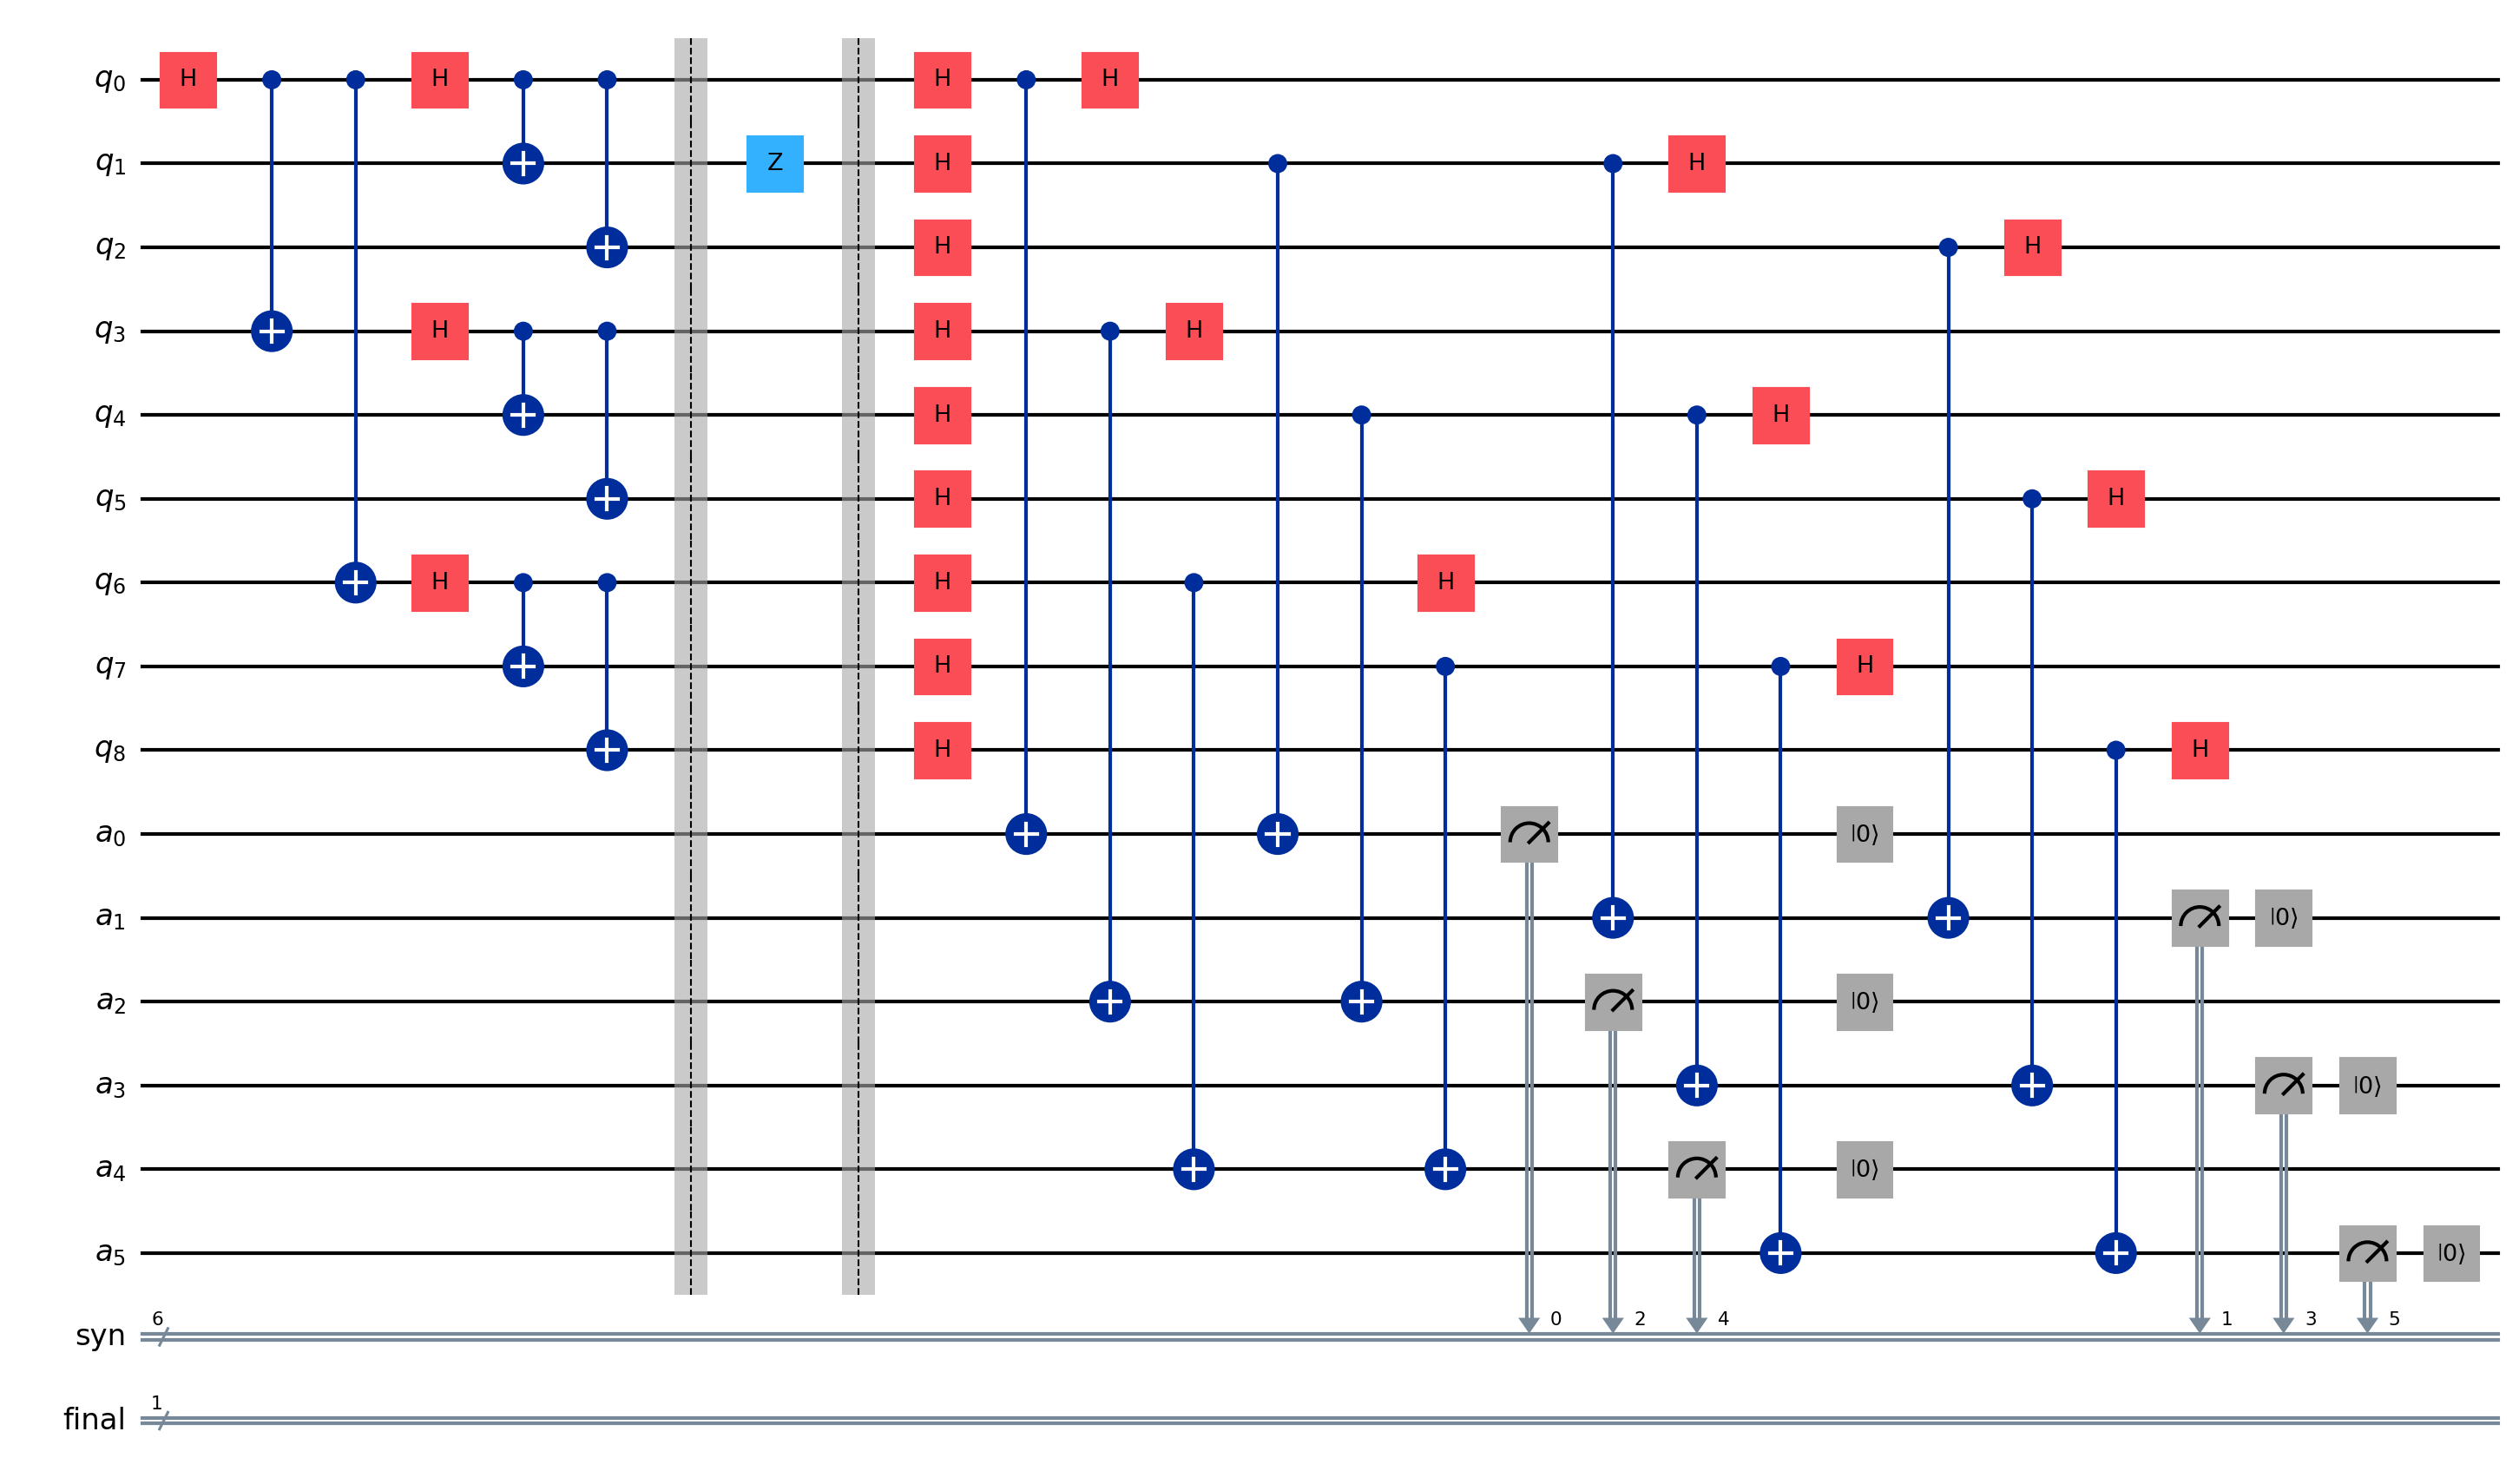
\includegraphics[width=0.45\textwidth]{../Codes/results/9bitCode/SyndromeMeasurementCircuit.png}
    \caption{Syndrome Measurement Circuit for 9-bit Code}
    \label{fig:9bitCodeResults}
\end{figure}
The first block encodes the qubit using CNOT and Hadamard gates. The second block adds the Z error in the 2nd qubit. The third block performs the syndrome measurement using 6 ancilla qubits. These measurements are then used to determine the error and correct it which is done in the next circuit.

\begin{figure}[h]
    \centering
    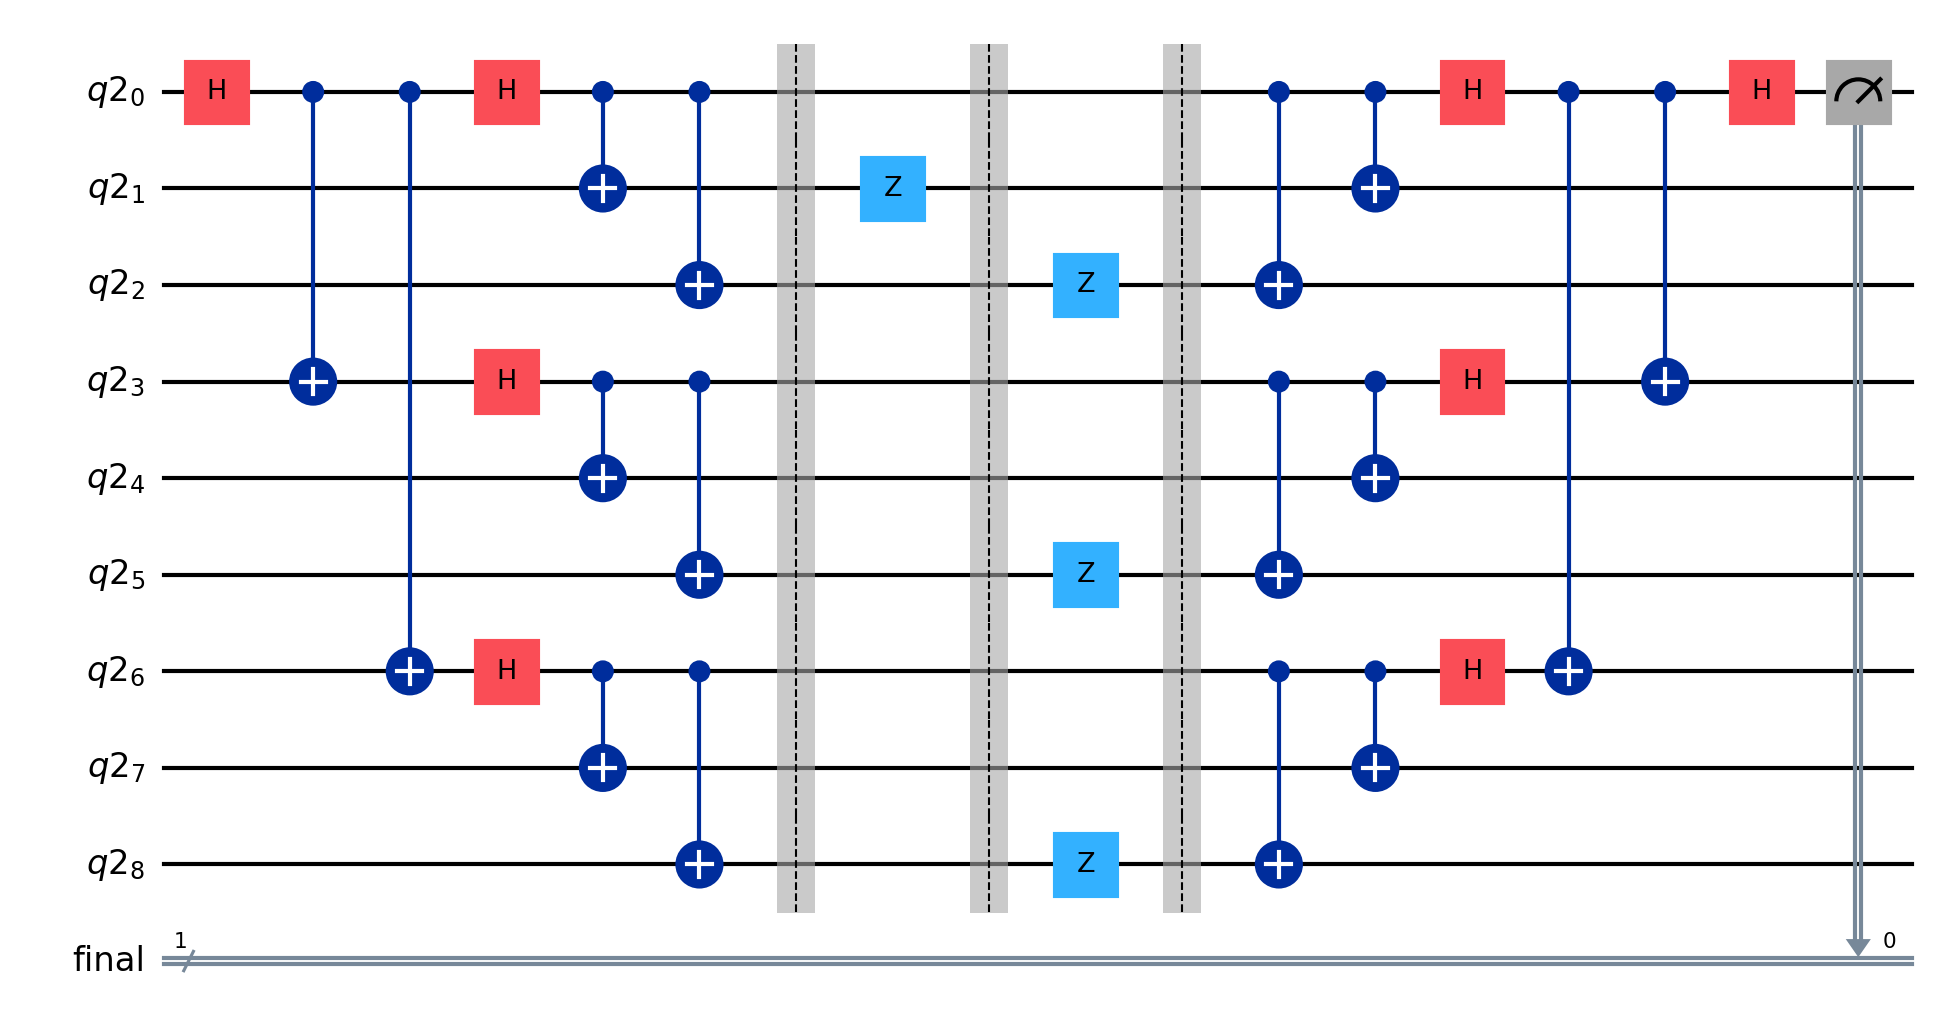
\includegraphics[width=0.45\textwidth]{../Codes/results/9bitCode/FinalCircuit.png}
    \caption{9-bit Shor Code Circuit for Z error}
    \label{fig:9bitCodeCircuit}
\end{figure}

The first two blocks are the same as above. The third block performs the error correction and the final block decodes the qubit back to a single qubit and measures it.

The results obtained are as follows:
\begin{figure}[h]
    \centering
    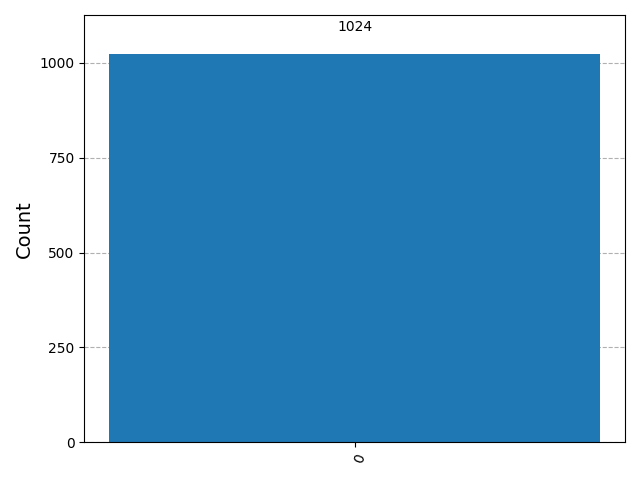
\includegraphics[width=0.45\textwidth]{../Codes/results/9bitCode/FinalHistogram.png}
    \caption{9-bit Code Results for Z error}
    \label{fig:9bitCodeResults}
\end{figure}

This histogram shows that the output is "0" with a probability of 1, indicating that the error correction was successful and the logical qubit was restored to its original state as the final measurement is done in the X-basis.
\section{Conclusion}
This is the conclusion.

\bibliographystyle{IEEEtran}
\bibliography{refs.bib}

\end{document}